\chapter{环面退化与镜像对称}
\SourcePage{81}
\section{Batyrev 镜像构造}
\subsection{反身多胞体}
\thmnum{definition}{1}\begin{definition}\label{def:5.1}
设 $\Xi\subset M_{\RR}$ 为满维格多胞体，且 $0$ 在其内部。若
\begin{enumerate}[label=(\roman*)]
\item $\Int(\Xi)\cap M=\{0\}$；
\item $\Xi$ 的每个侧面到原点的整仿射距离均为 $1$，
\end{enumerate}
则称 $\Xi$ 为\Term{fanshenduobaoti}{反身多胞体}。等价地，$\Xi$ 与 $\Xi^\circ$ 都是格多胞体。此时同时有
\begin{enumerate}[label=(\roman*)]
\item $\Int(\Xi)\cap M=\{0\}$；
\item $\Int(\Xi^\circ)\cap N=\{0\}$。
\end{enumerate}
\end{definition}
注意，$\Xi$ 反身当且仅当 $\Xi^\circ$ 反身。
\examnum{1}\begin{example}\label{ex:5.1}
令
\Eq{5.1}{\Xi=\vcenter{\hbox{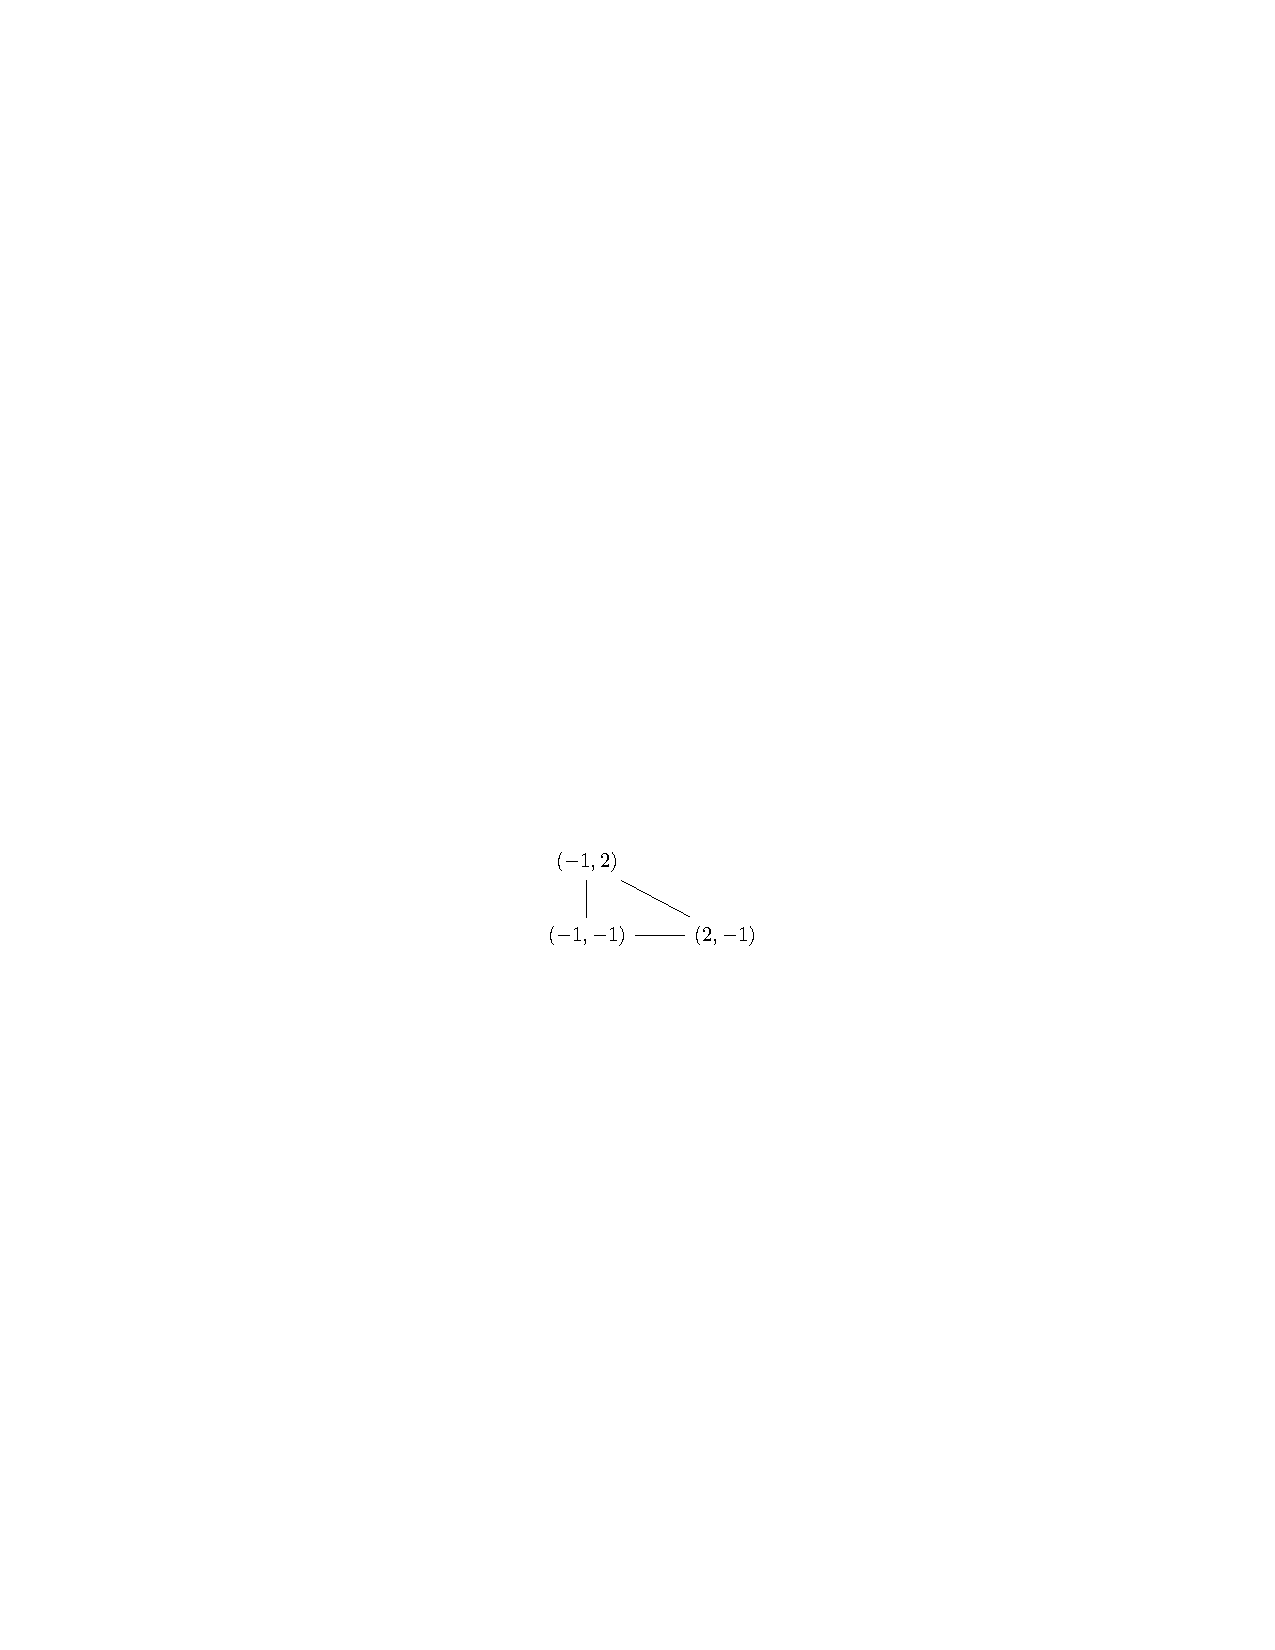
\includegraphics[width=0.2584\linewidth]{images/diagram-5-1.pdf}}}.}
则其对偶为
\Eq{5.2}{\Xi^\circ=\vcenter{\hbox{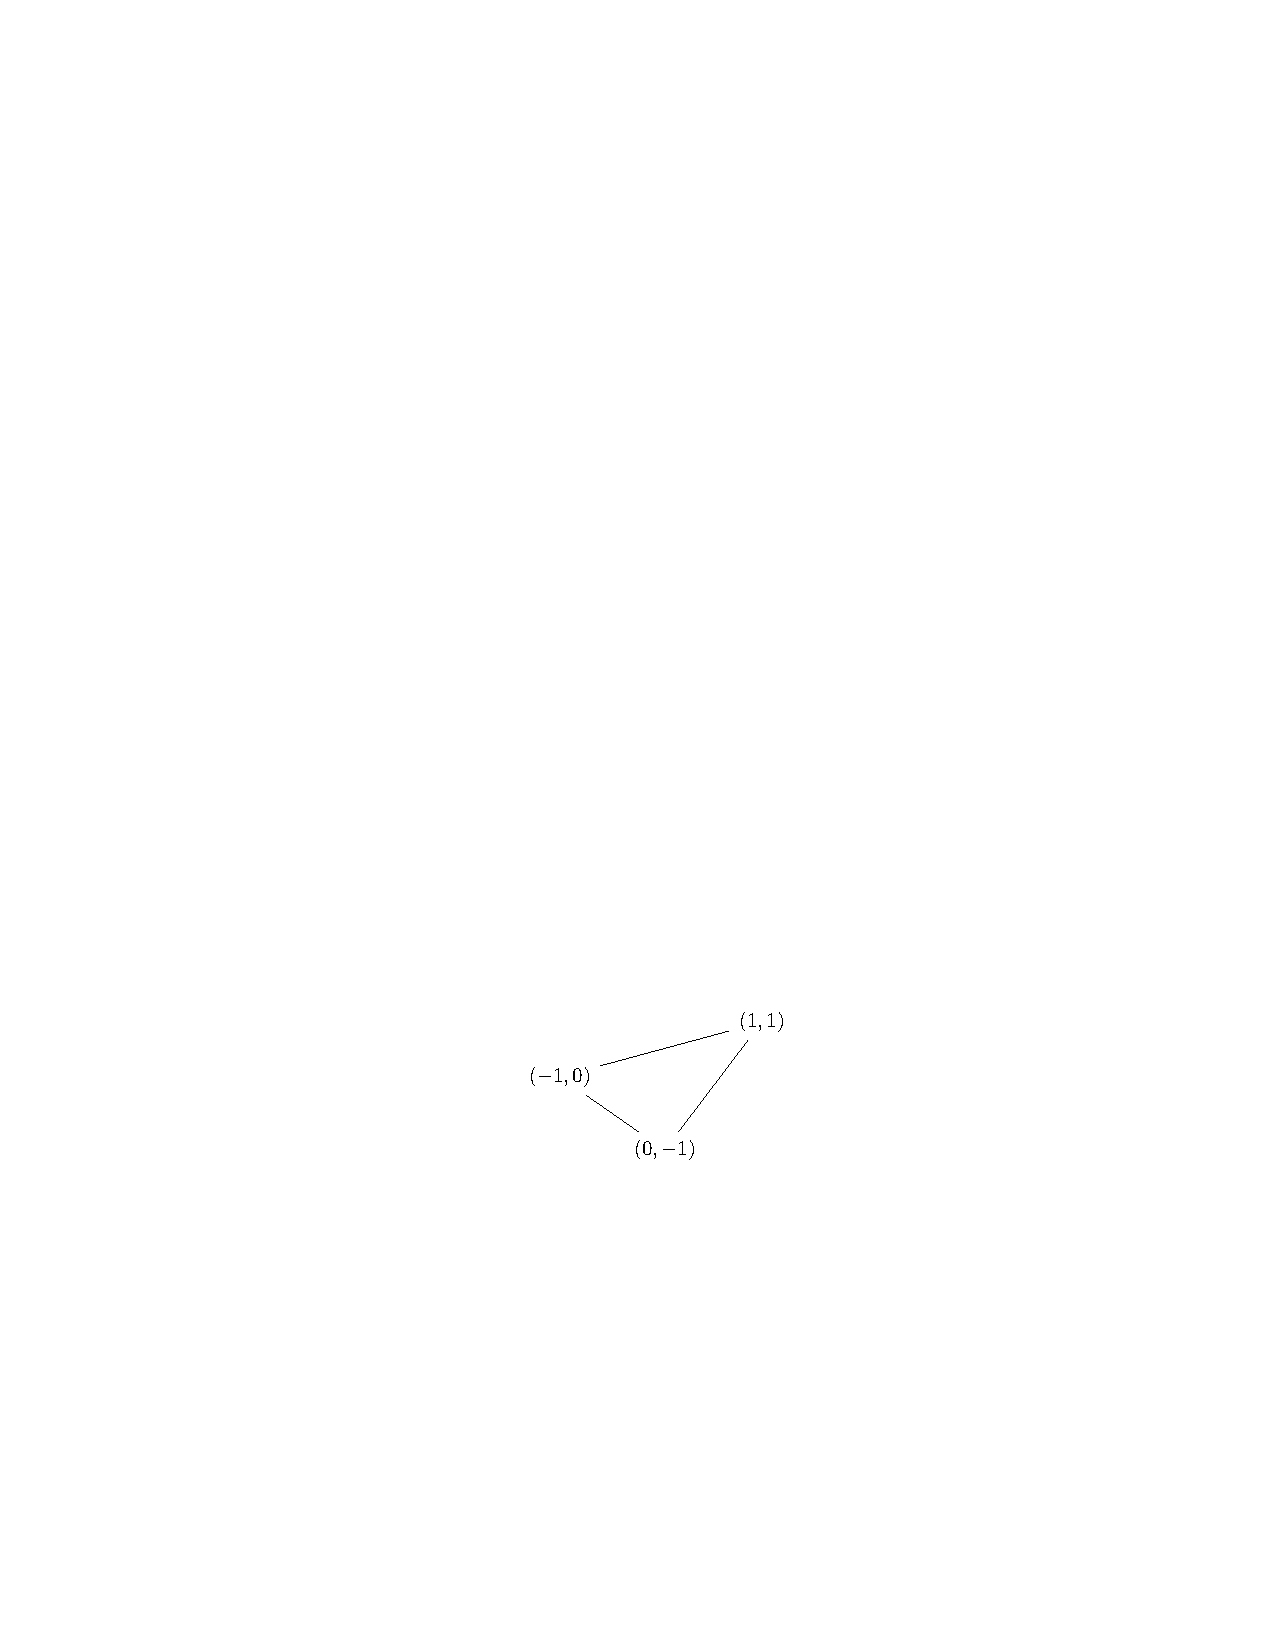
\includegraphics[width=0.3165\linewidth]{images/diagram-5-2.pdf}}}.}
二者都只有一个内部格点。
\end{example}
\examnum{2}\begin{example}\label{ex:5.2}
以原点为中心、边长为 $2$ 的正方形，其对偶可由它旋转 $45^\circ$ 并适当缩放得到。
\end{example}
二维中只有16个反身多胞体，见图~\ref{fig:5.1}。三维中有 $4319$ 个，四维中有 $473800776$ 个。人们说弦理论有许多不同的模型，就是由此而来。
\begin{Counterexample}{3}\label{counterex:3}
取 $(-1,-1),(-1,0),(1,0),(0,2)$ 的凸包，则它不是反身多胞体。
\end{Counterexample}
\SourcePage{82}
\OriginalFigure{fig-5-1.pdf}{0.5093}{二维的16个反身多胞体。原图来自文献~\cite{ref1}。}{fig:5.1}
\subsection{Fano 环面簇}
\thmnum{definition}{2}\begin{definition}\label{def:5.2}
若射影簇 $X$ 具有 Gorenstein 奇点，且反典范丛 $-K_X$ 丰，则称 $X$ 为 Fano 簇。对于此处考虑的正规 Cohen–Macaulay 环面簇，Gorenstein 条件等价于 $K_X$ 为 Cartier 除子，也等价于对偶化层为线丛。
\end{definition}
\thmnum{proposition}{1}\begin{proposition}\label{prop:5.1}
完备环面簇 $X$ 为 Fano 簇，当且仅当 $X\simeq X(\Sigma_\Xi)$，其中 $\Xi$ 反身。
\end{proposition}
\begin{proof}
令 $\Sigma$ 为 $N_{\RR}$ 中的扇。仿射坐标图 $U=\Spec k[\sigma^\vee\cap M]$ 的典范除子为 $K_U=-\sum_iD_i$，其中 $D_i$ 为环面素除子。全纯体积形式 $z_1^{-1}dz_1\wedge\cdots\wedge z_d^{-1}dz_d$ 沿每个环面除子都有一阶极点。

$K_U$ 为 Cartier 除子，当且仅当存在 $m_\sigma\in M$，使每条射线的本原生成向量 $v_i$ 都满足 $\langle m_\sigma,v_i\rangle=1$。把这一条件译成多胞体语言：$\Xi$ 是各 $m_\sigma$ 的凸包，而上述条件正是其侧面到原点的整距离为 $1$。
\end{proof}
\subsection{光滑情形中的 Calabi–Yau 超曲面}
设 $X$ 为光滑 Fano 簇，且 $\Gamma(X,-K_X)\ne0$。当反典范线性系无基点时，对一般截面 $s$，由 Bertini 定理，$Z(s)\subset X$ 光滑。伴随公式给出
\Eq{5.3}{K_{Z(s)}=(-K_X+K_X)|_{Z(s)}=0.}
问题在于，光滑 Fano 环面簇只有很少的几种。
\subsection{部分消解奇点}
记 $\Sigma_\Xi$ 为在 $\Xi^\circ$ 的各个面上取锥得到的扇。
\thmnum{definition}{3}\begin{definition}\label{def:5.3}
$\Sigma_\Xi$ 的一个极大、射影、保典范、部分细分，简称 MPCP 细分，是扇 $\Sigma$，满足：
\begin{itemize}
\item $\Sigma$ 是 $\Sigma_\Xi$ 的细分；
\item $\Sigma$ 单纯且射影；
\SourcePage{83}
\item 其射线的本原生成向量集合为
\Eq{5.4}{\Sigma(1)=\Xi^\circ\cap(N\setminus\{0\})=\partial\Xi^\circ\cap N.}
\end{itemize}
也就是说，要对 $\Xi^\circ$ 的每个面作使用全部边界格点的正则三角剖分。
\end{definition}
\begin{Note}{5.1}当 $d\ge3$ 时，$\Sigma$ 未必唯一，因为可能有许多不同的细分。\end{Note}
\thmnum{proposition}{2}\begin{proposition}\label{prop:5.2}
若 $\Sigma$ 是 MPCP 细分，则：
\begin{enumerate}[label=(\roman*)]
\item $X_\Sigma$ 是 Gorenstein 轨形；\footnote{在余维不超过3的点处光滑，但一般并非处处光滑。}
\item $\Xi$ 为与 $-K_{X_\Sigma}$ 关联的多胞体；
\item 诱导映射 $f:X_\Sigma\to X(\Sigma_\Xi)$ 保典范，即典范丛的拉回仍为典范丛：$K_{X_\Sigma}=f^*K_{X(\Sigma_\Xi)}$；
\item $-K_{X_\Sigma}$ 半丰，即由整体截面生成，而且是大的。\footnote{此处等价于 $(-K_{X_\Sigma})^d>0$。}
\end{enumerate}
\end{proposition}
\subsection{Batyrev 超曲面镜像}
设 $\Xi,\Xi^\circ$ 为一对反身多胞体，$\Sigma,\check\Sigma$ 分别为 $\Sigma_\Xi,\Sigma_{\Xi^\circ}$ 的 MPCP 细分。它们给出镜像对偶的族。对一般截面 $s\in\Gamma(X_\Sigma,-K_{X_\Sigma})$，构造
\Eq{5.5}{Z(s)\subset X_\Sigma.}
类似地，对 $\check s\in\Gamma(X_{\check\Sigma},-K_{X_{\check\Sigma}})$，构造
\Eq{5.6}{Z(\check s)\subset X_{\check\Sigma}.}
这些就是镜像对。注意，$\Gamma(X,-K_X)=\operatorname{Map}(\Xi\cap M,k)$。
\Lecture{23}{2019年11月19日}
\subsection{镜像定理}
\thmnum{theorem}{3}\begin{theorem}\label{thm:5.3}
若 $X$ 与 $\check X$ 均为光滑 Calabi–Yau 簇，则 $h^{1,1}(X)=h^{n-1,1}(\check X)$。
\end{theorem}
\begin{proof}见文献~\cite{ref6} 的定理4.15，或文献~\cite{ref2}。\end{proof}
\thmnum{theorem}{4}\begin{theorem}[Batyrev]\label{thm:5.4}
对于轨形奇点，存在 Hodge 数 $h^{p,q}$ 的“弦论”精化，满足
\Eq{5.7}{h^{p,q}_{\mathrm{st}}(X)=h^{n-p,q}_{\mathrm{st}}(\check X).}
\end{theorem}
这与动机积分有关。另外，Gromov–Witten 理论与镜像侧的 Hodge 结构变分相对应。
\thmnum{theorem}{5}\begin{theorem}\label{thm:5.5}
$\mathrm{GW}_{g=0}(X)=\mathrm{VHS}(\check X)$。
\end{theorem}
\begin{proof}见文献~\cite{ref5,ref12,ref22}。\end{proof}
还存在由 Batyrev–Borisov 给出的环面完全交推广。接下来的目标，是作出更内蕴的构造，以适用于更一般的情形；这正是文献~\cite{ref15,ref17} 中正在开展的研究。
\examnum{3}\begin{example}\label{ex:5.3}
考虑图~\ref{fig:5.2} 中的多胞体，按图右侧给顶点及格点标上单项式。这样便在 $\PP^2\times\mathbb A_t^1$ 中得到退化族
\Eq{5.8}{xyz+t^2(x^2y+xy^2+y^2z+yz^2+x^2z+xz^2)+t^3(x^3+y^3+z^3)=0.}
对一般非零 $t$，它是 Calabi–Yau 超曲面，即椭圆曲线；$t=0$ 时，$xyz=0$ 是三个超平面 $\PP^1$ 的并。
\end{example}
\SourcePage{84}
\OriginalFigure{fig-5-2.pdf}{0.5328}{多胞体及其唯一的 MPCP 细分；标注的数值给出一个分段线性函数。}{fig:5.2}
\OriginalFigure{fig-5-3.pdf}{0.8535}{从 $\Omega$ 出发构造族 $\mathcal X$。}{fig:5.3}
考虑 $\mathcal X\to S$，在变形理论中 $S$ 可以是某个离散赋值环的谱；实际上也可以取局部环或完备局部环的谱。我们希望零点上的纤维 $X_0$ 是若干环面簇的并，即把环面簇沿余维一分层作纤维余积粘合起来。
\section{Mumford 型环面退化}
\subsection{构造}
设 $\Omega\subset N_{\RR}$ 凸且闭。取有理多面体分解 $\mathscr P=\{\sigma\}$，使
\Eq{5.9}{\Omega=\bigcup_{\sigma\in\mathscr P}\sigma,}
此分解局部有限，且各胞腔沿共同的面相交。由此得到扇
\Eq{5.10}{\Sigma_{\mathscr P}=\{C(\sigma)\subset N_{\RR}\oplus\RR:\sigma\in\mathscr P\}\cup\{\text{这些锥的所有面}\}.}
其想法是把 $\Omega$ 放在高度一处，再像图~\ref{fig:5.3} 那样取锥。高度投影诱导 $\pi:X(\Sigma_{\mathscr P})\to\mathbb A^1$。
\thmnum{proposition}{6}\begin{proposition}\label{prop:5.6}
\begin{enumerate}[label=(\alph*)]
\item $\pi^{-1}(\mathbb A^1\setminus\{0\})\simeq(\mathbb A^1\setminus\{0\})\times X(\Sigma_{\mathscr P}\cap(N_{\RR}\times\{0\}))$，总维数为 $d+1$。
\item
\Eq{5.11}{\pi^{-1}(0)=\bigcup_{v\text{ 为 }\mathscr P\text{ 的顶点}}\underbrace{X((\Sigma_{\mathscr P})_v)}_{D_v}.}
\item
\Eq{5.12}{\operatorname{mult}_{D_v}(\pi^{-1}(0))=\min\{d\in\NN\setminus\{0\}:dv\in N\}.}
\end{enumerate}
\end{proposition}
\SourcePage{85}
\begin{proof}
(a) $\pi^{-1}(\mathbb A^1\setminus\{0\})$ 对应于 $N\oplus\ZZ$ 中的扇 $\{C(\sigma)\cap(N_{\RR}\times\{0\})\}$。
(b) $\pi^{-1}(0)$ 是那些映到 $\mathbb A^1$ 原点的环面素除子 $D_w$ 的并，其对应射线 $w$ 在高度投影下非零。
(c) 射线由本原格向量 $(n,d)$ 生成，其中 $v=n/d$，$d>0$ 最小。由单项式的阶数公式，
\Eq{5.13}{\operatorname{ord}_{D_w}\pi^*(t)=d.}
\end{proof}
在图~\ref{fig:5.3} 的例子中，$t\ne0$ 时 $\pi^{-1}(t)=\PP^2$；$t=0$ 时，
\Eq{5.14}{\pi^{-1}(0)=\bigcup_{i=1}^3X\left(\vcenter{\hbox{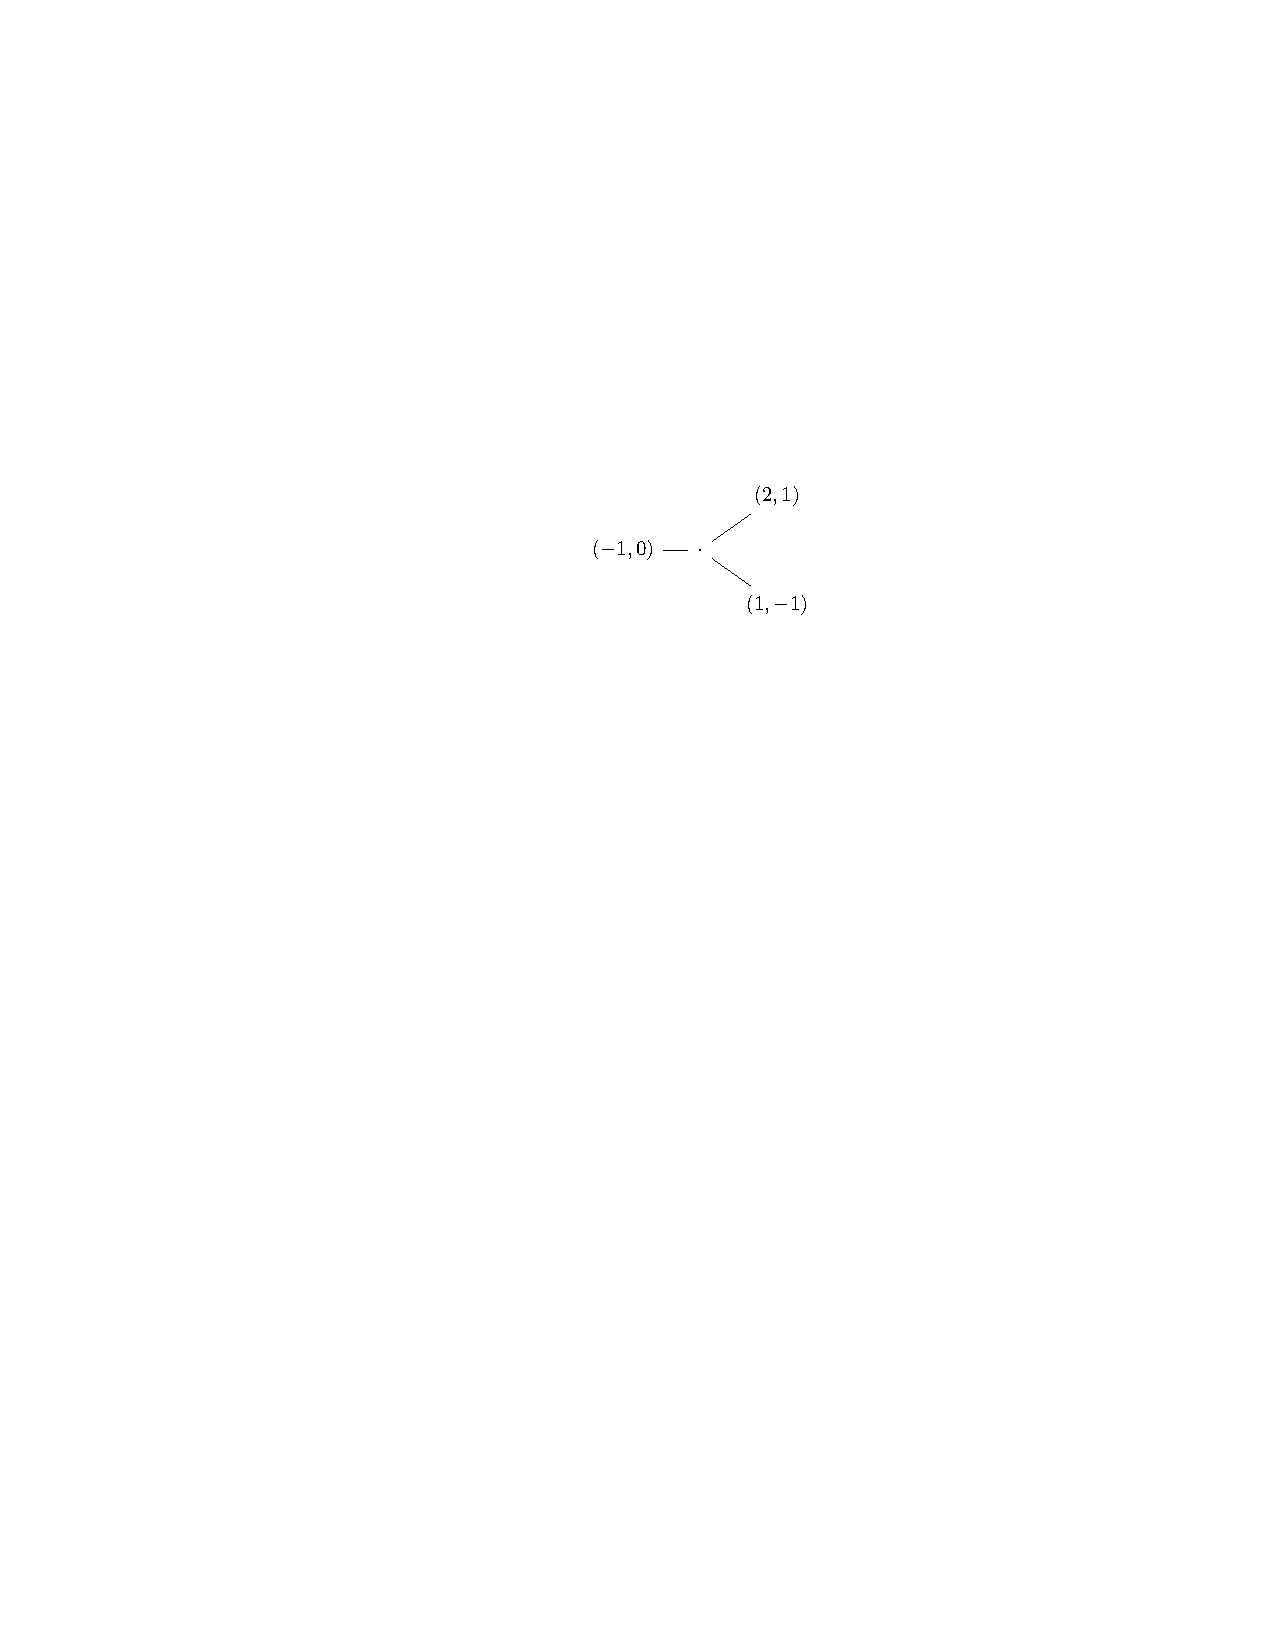
\includegraphics[width=0.2677\linewidth]{images/diagram-5-14.pdf}}}\right).}
注意，每个不可约分支都满足
\Eq{5.15}{\PP^2\xrightarrow{/\,(\ZZ/3)}D_v\simeq\PP(1,1,3).}
\subsection{多胞体图景}
镜像对称需要带极化的版本。对有理多面体 $\Xi\subset M_{\RR}$，记其有理多面体分解为 $\check{\mathscr P}$。若细分正则，则在适当放大后，存在整分段仿射严格凸函数 $\check\varphi:\Xi\to\RR$。其图像为 $\Gamma_{\check\varphi}\subset M_{\RR}\times\RR$，上方凸包为
\Eq{5.16}{B_{\check\varphi}=\Gamma_{\check\varphi}+(0\oplus\RR_{\ge0})=\{(m,h)\in\Xi\times\RR:h\ge\check\varphi(m)\}.}
由此得到带极化的 Mumford 退化
\Eq{5.17}{X(\Sigma_{B_{\check\varphi}}),}
其中，
\Eq{5.18}{X(\Sigma_{B_{\check\varphi}})\simeq\operatorname{Proj}k[C(B_{\check\varphi})\cap(M\oplus\ZZ\oplus\ZZ)].}
\subsection{Mumford 退化的镜像对称}
其思想是如下的一一对应：
\Eq{5.19}{\begin{aligned}(B=|\mathscr P|,\mathscr P,\varphi)&\longleftrightarrow(\check B=|\check{\mathscr P}|,\check{\mathscr P},\check\varphi),\\\text{分段仿射函数}&\longmapsto\check\sigma=\text{$\varphi|_{\Sigma_\sigma}$ 的 Newton 多面体},\quad\sigma\in\mathscr P,\\(\Sigma_{\mathscr P},\psi)&\longleftrightarrow(\Xi,\check\psi),\end{aligned}}
其中 $\psi$ 为分段线性函数。
\examnum{4}\begin{example}\label{ex:5.4}
图~\ref{fig:5.4} 的 $\mathscr P$ 给出 $\PP^2$ 的一个环面退化；图中还画出了对应的 $\check{\mathscr P}$。
\end{example}
\Lecture{24}{2019年11月21日}
\SourcePage{86}
\OriginalFigure{fig-5-4.pdf}{0.9579}{一个 $\mathscr P$ 与 $\check{\mathscr P}$ 的例子。}{fig:5.4}
\subsection{环面退化}
于是有
\Eq{5.20}{\begin{tikzcd}X_0\arrow[r,hook]\arrow[d]\&(\mathcal X,\mathcal L)\arrow[d,"{\pi}"]\\0\arrow[r,hook]\&S_t=\Spec(\text{离散赋值环}),\end{tikzcd}}
其中希望 $X_0$ 是射影环面簇的并，且 $\mathcal L|_{P(\sigma)}=\OO_{P(\sigma)}(1)$。相应数据为 $(B=\bigcup\sigma,\mathscr P=\{\sigma\},\varphi)$，其中 $B$ 是带边界流形，$\dim_{\RR} B=\dim X=d$，$\varphi$ 为极化函数。这是扇的图景；$\varphi$ 对应于 $\pi$ 在余维一处的环面模型。

还存在等价的多面体构造。\Term{lisanlegendre}{离散 Legendre 变换}就是数据 $(B,\mathscr P,\varphi)$ 的镜像对偶，产生 $(\check B,\check{\mathscr P},\check\varphi)$。
\section{走向 Gross–Siebert 型环面退化}
\subsection{Dwork 族与\texorpdfstring{$A_1$}{A₁}奇点}
考虑
\Eq{5.21}{\mathcal X=Z\left(t\sum_{i=0}^3z_i^4+\prod_{i=0}^3z_i\right)\subset\PP^3\times\mathbb A^1,}
并投影到 $\mathbb A^1$。这是课程开头五次超曲面族的低一维对应，给出 K3 曲面的退化。$X_0=\pi^{-1}(0)$ 是四个 $\PP^2$ 的并，各个 $\PP^2$ 由极大胞腔对应的 $P(\sigma)$ 给出。总空间 $\mathcal X$ 在 $X_0$ 的奇异轨迹上有 $6\cdot4=24$ 个三维 $A_1$ 奇点；这个轨迹由6条 $\PP^1$ 组成。

在 $z_0,z_1\ne0$ 处，以 $z_0=1$ 去齐次化，得到局部方程
\Eq{5.22}{z_2z_3=-t\,\frac{1+z_1^4+z_2^4+z_3^4}{z_1}.}
在奇点附近作解析坐标变换后，它同构于 $uv=wt$，即一个 $A_1$ 奇点。模 $t^{k+1}$ 后，
\Eq{5.23}{\mathcal X\bmod t^{k+1}=\bigcup_{i=0}^3X_{\sigma_i}^k,}
其中 $X_{\sigma_i}^0=P(\sigma_i)$。这些对象本质上是 $X_{\sigma_i}\subset\mathcal X$ 的 $k$ 阶邻域。观察到，各个局部模型
\SourcePage{87}
完全由 $(B,\mathscr P,\varphi)$ 决定；只有更高余维处的识别不是环面的，即粘合并非环面粘合。
\subsection{关键例子：一个\texorpdfstring{$A_1$}{A₁}奇点}
考虑两个胞腔 $\sigma_1,\sigma_2$，它们都是半平面，交于实直线 $\rho$。把交集上的坐标记为 $w$，$\sigma_1$、$\sigma_2$ 的横向坐标分别记为 $u,v$。我们希望交集上的 $w=-1$ 处出现一个 $A_1$ 奇点。因此取
\Eq{5.24}{uv=\underbrace{(1+w)}_{f_\rho}\,t\pmod{t^{k+1}}.}
要粘合的环面模型为
\Eq{5.25}{R_{\sigma_1}=\CC[u,v,w^{\pm1},t]/(uv-t,t^{k+1},v^{k+1}),}
\Eq{5.26}{R_{\sigma_2}=\CC[u,v,w^{\pm1},t]/(uv-t,t^{k+1},u^{k+1}).}
相交处的模型为 $X_\rho^k=\Spec R_{\rho,\sigma_i}$。在 $f_\rho$ 可逆的开集上，粘合图为
\Eq{5.27}{\begin{gathered}R_{\sigma_1}[f_\rho^{-1}]\longrightarrow R_{\rho,\sigma_1}=(R_{\sigma_1}/(u^{k+1}))[f_\rho^{-1}],\\R_{\sigma_2}[f_\rho^{-1}]\longrightarrow R_{\rho,\sigma_2}=(R_{\sigma_2}/(v^{k+1}))[f_\rho^{-1}],\\R_{\rho,\sigma_1}\xrightarrow{\sim}R_{\rho,\sigma_2},\qquad u\longmapsto f_\rho u,\quad v\longmapsto f_\rho^{-1}v.\end{gathered}}
反向识别把 $u$ 映为 $f_\rho^{-1}u$，$v$ 映为 $f_\rho v$。于是取纤维积得到
\Eq{5.28}{\begin{aligned}R_{\sigma_1}[f_\rho^{-1}]\times_{R_{\rho,\sigma_i}}R_{\sigma_2}[f_\rho^{-1}]&\simeq\left(\frac{\CC[u,v,w^{\pm1},t]}{uv-(1+w)t,\ t^{k+1}}\right)_{f_\rho},\\u&\longmapsto(u,f_\rho u),\\v&\longmapsto(f_\rho v,v),\\w&\longmapsto(w,w).\end{aligned}}

因此，在余维二轨迹之外，我们有由 $(B,\mathscr P,\varphi)$ 给出的两类环面模型。对于极大胞腔 $\sigma$，
\Eq{5.29}{R_\sigma^k=A_k[\Lambda_\sigma],}
其中 $A_k=\CC[t]/(t^{k+1})$，$\Lambda_\sigma\simeq\ZZ^d$ 是 $\sigma$ 所在的整切格。可把其中的元素理解为 $\sigma$ 上的整切向量。对于余维一胞腔 $\rho\in\mathscr P[d-1]$，
\Eq{5.30}{R_\rho^k=A_k[\Lambda_\rho][Z_+,Z_-]/(Z_+Z_--f_\rho t^{\kappa_\rho(\varphi)}),}
其中 $\kappa_\rho(\varphi)\in\NN\setminus\{0\}$ 是 $\varphi$ 沿 $\rho$ 的折角，$f_\rho\in A_k[\Lambda_\rho]$。这就是所谓数据位于一面壁上的含义。
\section{重构}
问题是如何从 $(B,\mathscr P,\varphi)$ 得到族 $\mathcal X\to S$。我们将把 $\Spec R_\sigma^k$ 与 $\Spec R_\rho^k$ 作纤维余积粘合，以构造 $\mathcal X$。具体的初始数据为
\Eq{5.31}{\left(B=\bigcup_{\sigma\in\mathscr P}\sigma,\ \mathscr P,\ \varphi,\ f_\rho\in A_k[\Lambda_\rho]\right).}
\SourcePage{88}
\subsection{不涉及散射的说明}
顶点 $v_1$ 处的扇结构为
\Eq{5.32}{\vcenter{\hbox{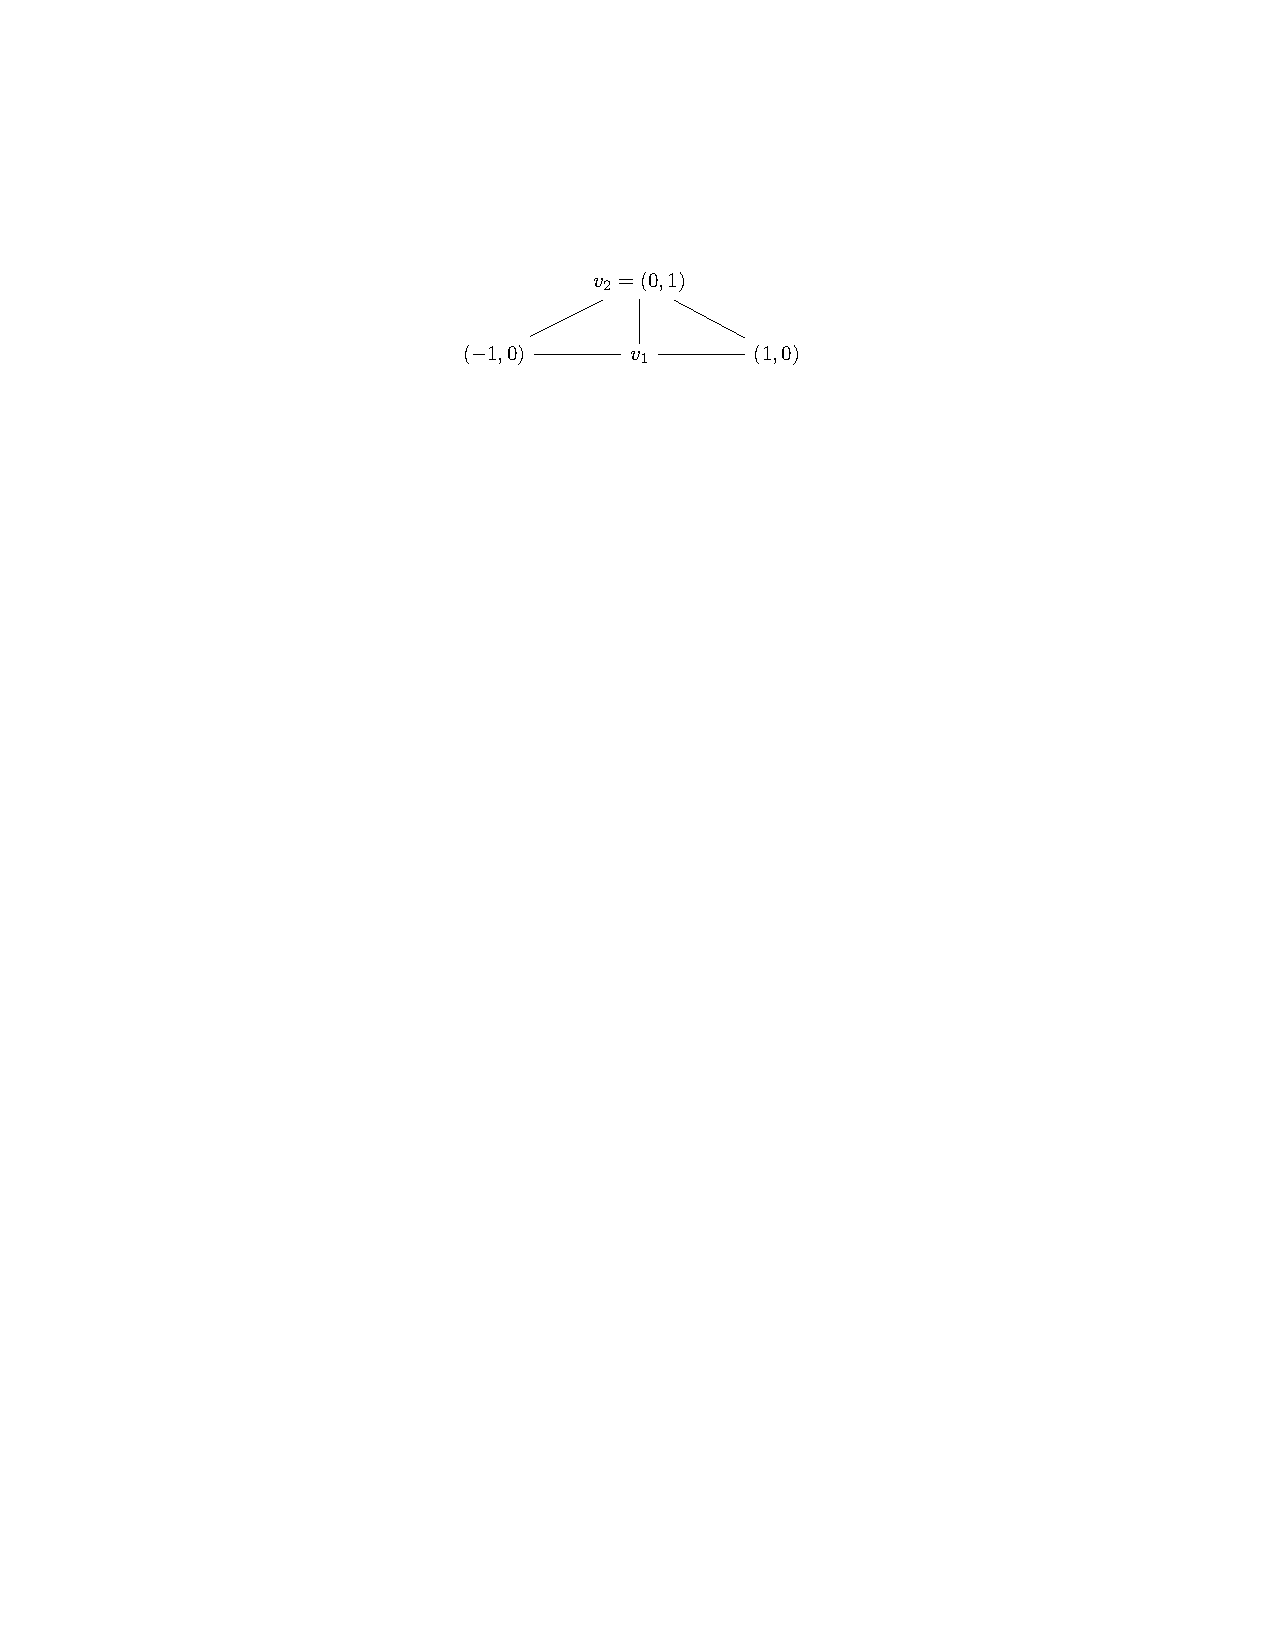
\includegraphics[width=0.4141\linewidth]{images/diagram-5-32.pdf}}}.}
顶点 $v_2$ 处的扇结构为
\Eq{5.33}{\vcenter{\hbox{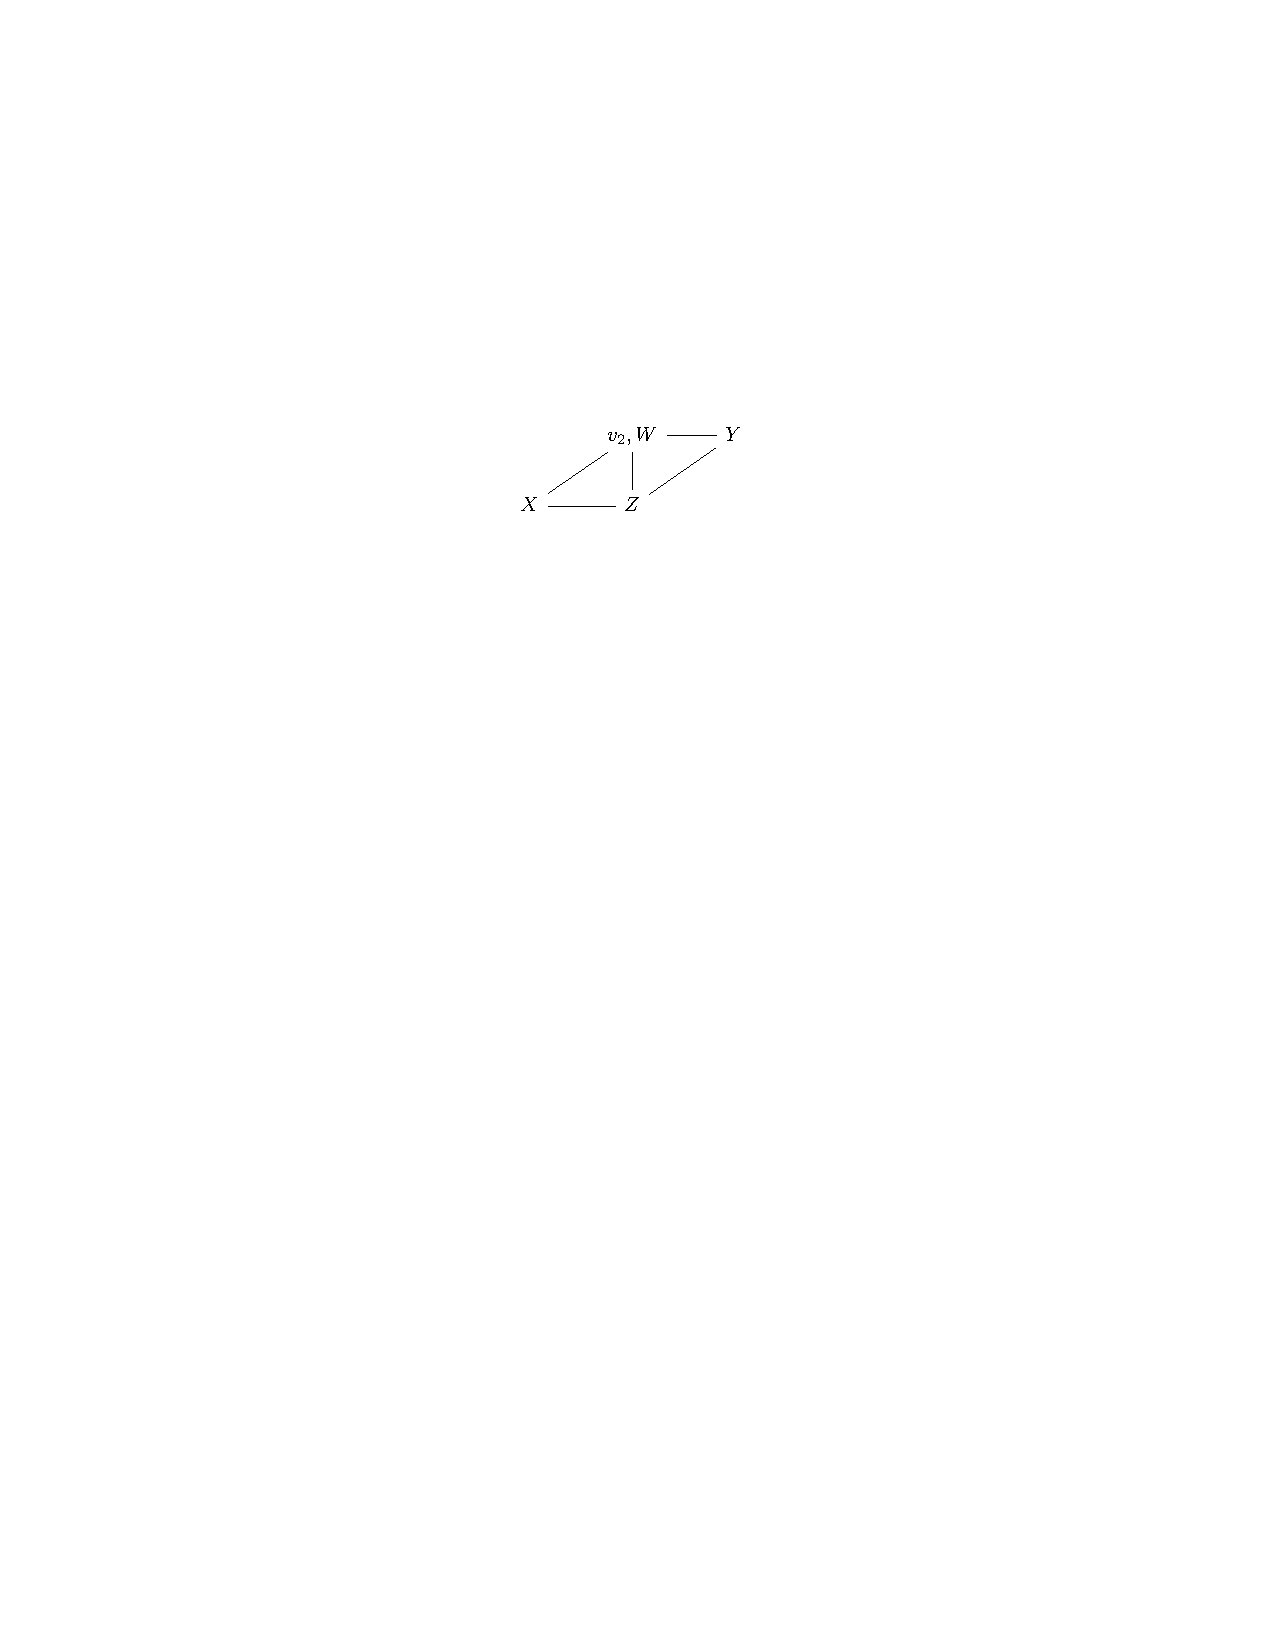
\includegraphics[width=0.2786\linewidth]{images/diagram-5-33.pdf}}}.}
这些结构给出不同的仿射结构。删去内部边上的一个点，就能处理这种差异。这里取
\Eq{5.34}{f_{\rho,v_1}=\alpha+w,}
其中 $\alpha\in\CC^\times$、$w=W/Z$。对 $R_{\rho,v_1}^k$，有
\Eq{5.35}{Z_+=y=Y/Z,}
\Eq{5.36}{Z_-=x=X/Z,}
以及方程
\Eq{5.37}{Z_+Z_-=(\alpha+w)t.}
齐次化得到
\Eq{5.38}{\frac YZ\frac XZ=\left(\alpha+\frac WZ\right)t.}
这给出一个非环面的二次曲线退化族。若采用 Mumford 型退化，则 $\alpha Z+W$ 会被单项式 $W$ 代替。

类似地，在 $R_{\rho,v_2}^k$ 的坐标中，令 $y=Y/W$、$x=X/W$、$z=Z/W$，有
\Eq{5.39}{Z_+=y=\frac YW,\qquad Z_-=xz^{-1}=\frac XW\frac WZ=\frac XZ.}
于是
\Eq{5.40}{Z_+Z_-=(z\alpha+1)t.}
齐次化后，
\Eq{5.41}{\frac YW\frac XZ=\left(\frac ZW\alpha+1\right)t,}
因此
\Eq{5.42}{XY=(Z\alpha+W)Zt.}
最终得到相容的模型
\Eq{5.43}{f_{\rho,v_1}=z^{m^\rho_{v_1,v_2}}f_{\rho,v_2},}
其中 $m^\rho_{v_1,v_2}\in\Lambda_\rho$。在本例中，$m^\rho_{v_1,v_2}=(0,1)$。将它加入初始数据，得到
\Eq{5.44}{(B,\mathscr P,\varphi,\{f_{\rho,v}\}).}
\SourcePage{89}
\subsubsection{传播}
考虑四个象限的副本粘合在一起：
\Eq{5.45}{\vcenter{\hbox{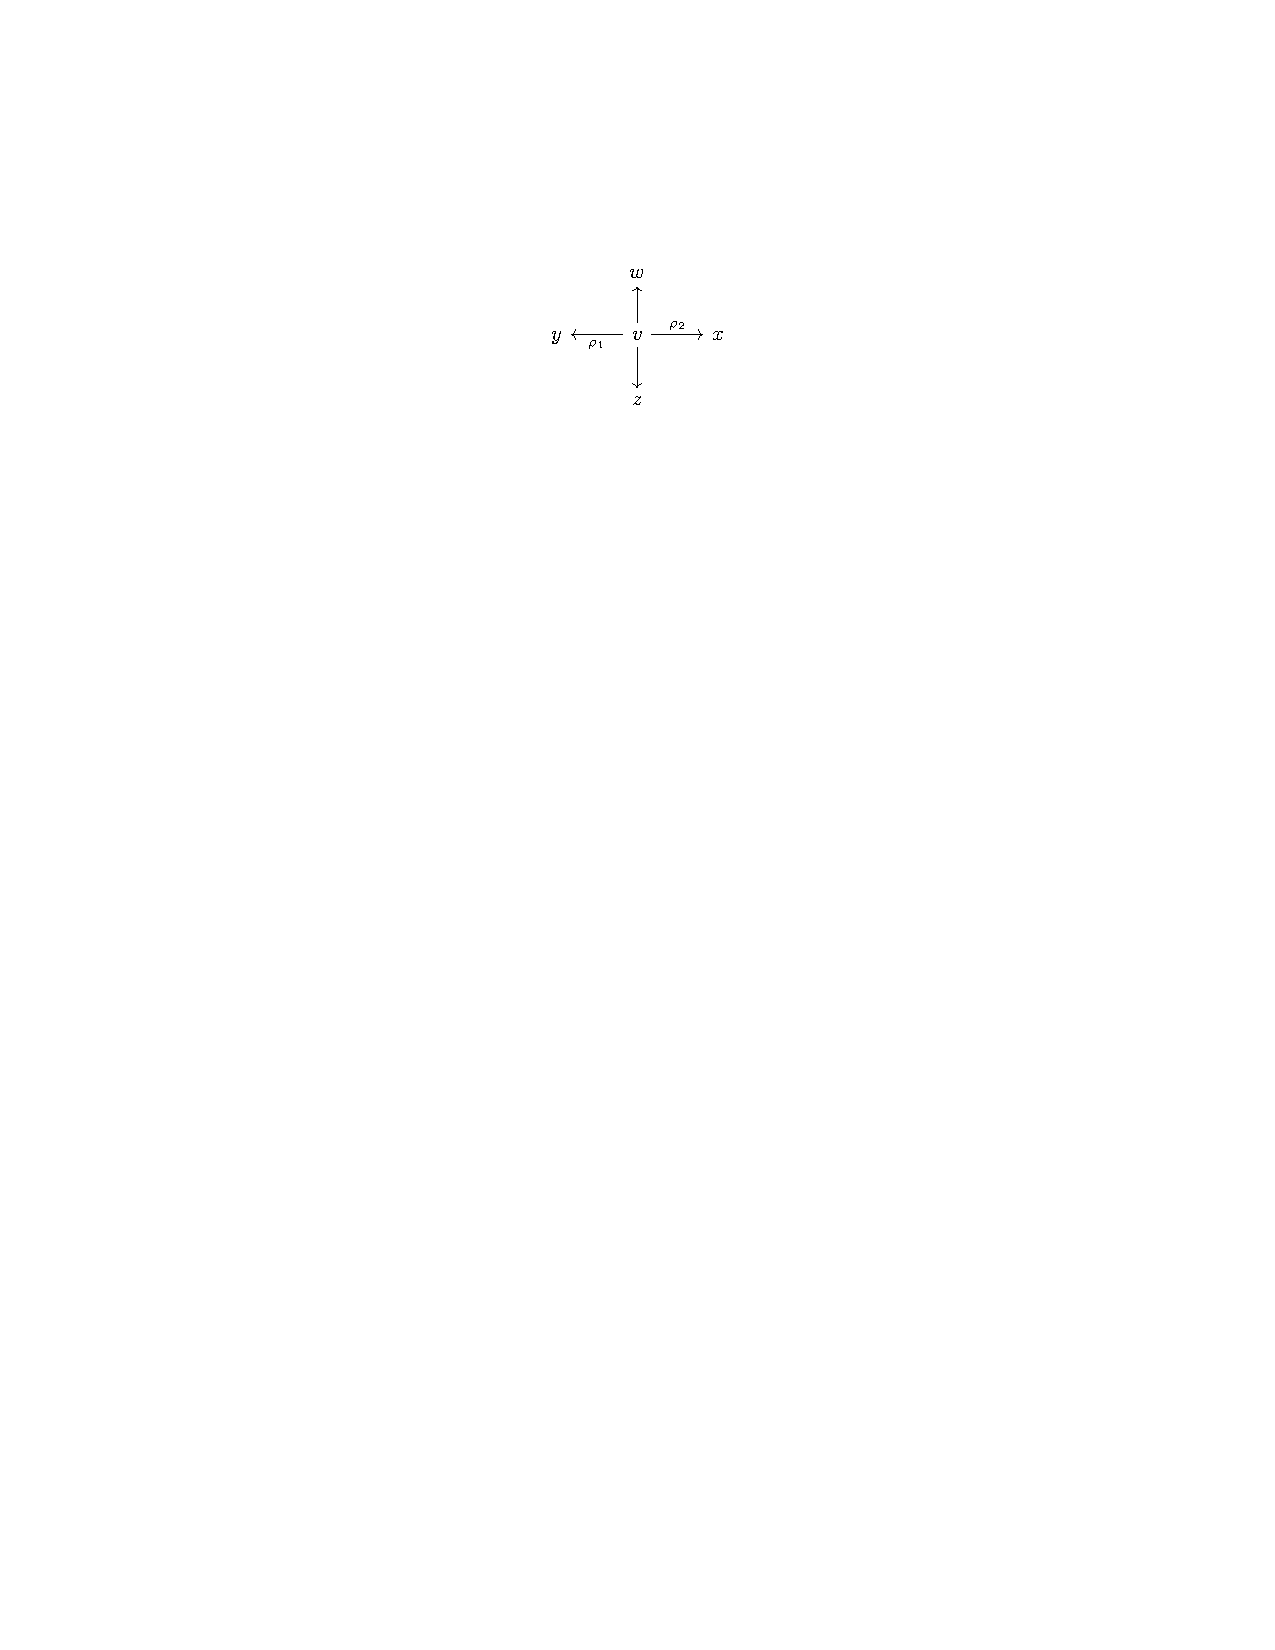
\includegraphics[width=0.2197\linewidth]{images/diagram-5-45.pdf}}}.}
顶点 $v$ 处的环面模型为
\Eq{5.46}{A_k[x,y,z,w]/(xy-t,zw-t).}
现在取 $f_{\rho_1}=1+y$。$R_{\rho_1}^k$ 的局部模型为 $zw=(1+y)t$。当 $x\ne0$ 时，$y=x^{-1}t$，所以必须有局部模型
\Eq{5.47}{zw=(1+x^{-1}t)t.}
这迫使我们令
\Eq{5.48}{f_{\rho_2}=1+x^{-1}t.}
可把这一过程理解为：每面壁都携带一个单项式的数据。
\subsubsection{离开余维一轨迹的壁}
\Eq{5.49}{\vcenter{\hbox{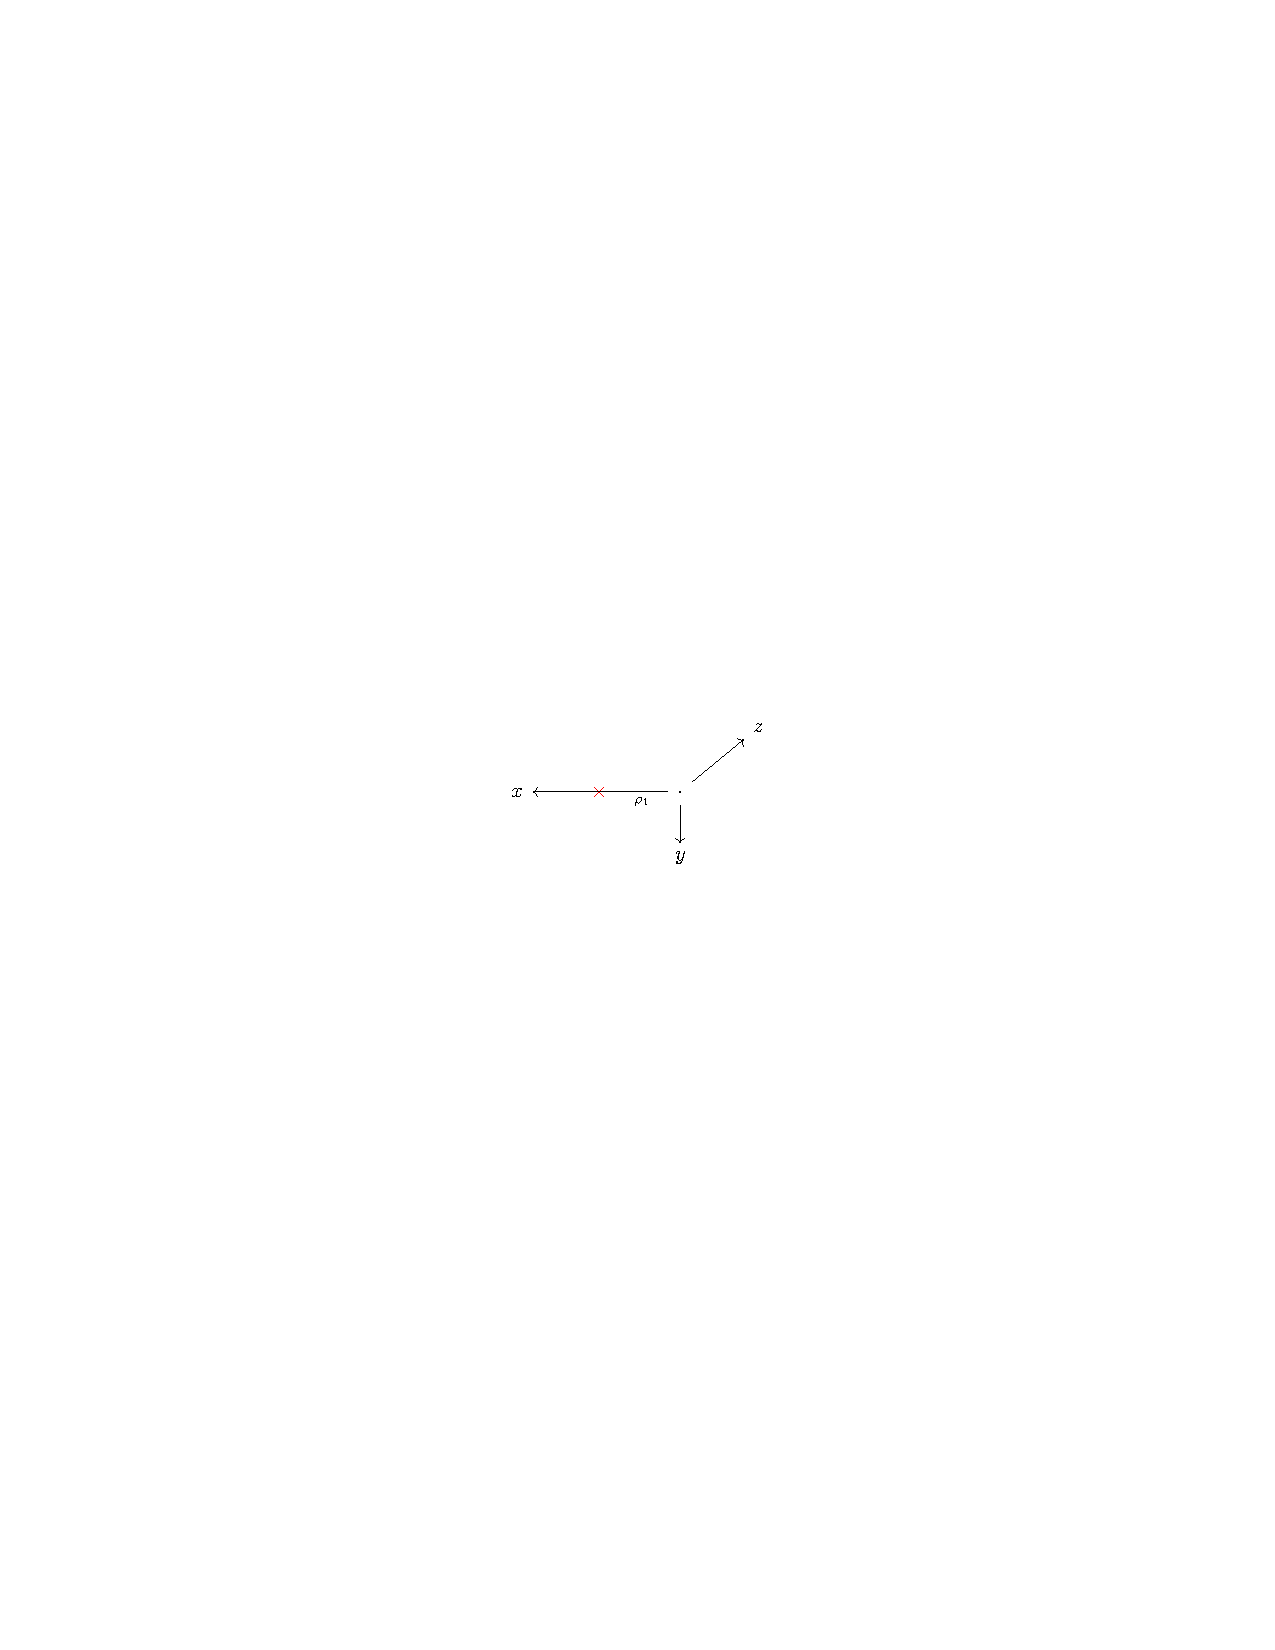
\includegraphics[width=0.3157\linewidth]{images/diagram-5-49.pdf}}}.}
环面模型为 $xyz=t$，且
\Eq{5.50}{f_{\rho_1}=1+x=1+(yz)^{-1}t.}
为了使它相容，取两个 $R_\sigma^k$ 的副本，并用一个非环面的“壁穿越”自同构 $\Phi$ 粘合。具体地，
\Eq{5.51}{\begin{aligned}y&\xmapsto{\Phi}(1+y^{-1}z^{-1}t)y,\\z&\xmapsto{\Phi}\underbrace{(1+y^{-1}z^{-1}t)^{-1}}_{\equiv1\pmod t}\,z.\end{aligned}}
\Lecture{25}{2019年11月26日}
\section{壁结构}
\subsection{壁}
固定 $k$，令 $A=\CC[t]/(t^{k+1})$；最终将令 $k\to\infty$。与往常一样，初始数据为
\Eq{5.52}{\left(B=\bigcup_{\sigma\in\mathscr P}\sigma,\ \mathscr P=\{\sigma\},\ \varphi\right),}
其中 $B$ 带有整仿射结构。奇异轨迹 $\Delta\subset B$ 的实余维为 $2$。
\thmnum{definition}{4}\begin{definition}\label{def:5.4}
$B$ 上的一面\Term{bi}{壁} $\mathfrak p$ 由以下数据组成：
\SourcePage{90}
\begin{itemize}
\item 有理多面体子集 $\mathfrak p\subseteq\sigma$，其中 $\dim\sigma=d$、$\dim\mathfrak p=d-1$，且 $\Int(\mathfrak p)\cap\Delta=\varnothing$；
\item 函数 $f_{\mathfrak p}=\sum_mc_mz^m$，其中 $m\in\Lambda_{\mathfrak p}\subset\Lambda_\sigma\simeq\ZZ^d$、$c_m\in A$。
\end{itemize}
\end{definition}
在余维零处，即 $\mathfrak p\cap\Int(\sigma)\ne\varnothing$ 时，有 $f_{\mathfrak p}=1+c_mz^m$，且 $c_m\equiv0\pmod t$。$m$ 给出传播方向；这种壁称为真壁。在余维一处，即 $\mathfrak p\subseteq\rho$、$\dim\rho=d-1$ 时，采用来自 $\rho$ 的函数 $f_{\mathfrak p}=f_\rho$，这种壁称为\Term{biban}{壁板}。对有限的 $k$，\Term{bijiegou}{壁结构} $\mathscr S$ 是壁的有限集合。
\subsection{壁穿越}
设 $(\mathfrak p,f_{\mathfrak p})$ 为余维零处的壁，$\mathfrak p\subset\sigma$。记
\Eq{5.53}{R_\sigma=A[\Lambda_\sigma]\simeq A[z_1^{\pm1},\ldots,z_d^{\pm1}].}
壁定义一个自同构
\Eq{5.54}{\Theta_{\mathfrak p}:R_\sigma\longrightarrow R_\sigma,}
其作用为
\Eq{5.55}{z^m\longmapsto f_{\mathfrak p}^{\langle n_{\mathfrak p},m\rangle}z^m,}
其中 $n_{\mathfrak p}\in\Lambda_\sigma^*$ 为按穿越方向选择的本原法向余向量，$n_{\mathfrak p}^\perp=\Lambda_{\mathfrak p}$。由于 $\Theta_{\mathfrak p}\equiv\id\pmod t$，它确实是自同构。
\examnum{5}\begin{example}\label{ex:5.5}
考虑如下壁：
\Eq{5.56}{\vcenter{\hbox{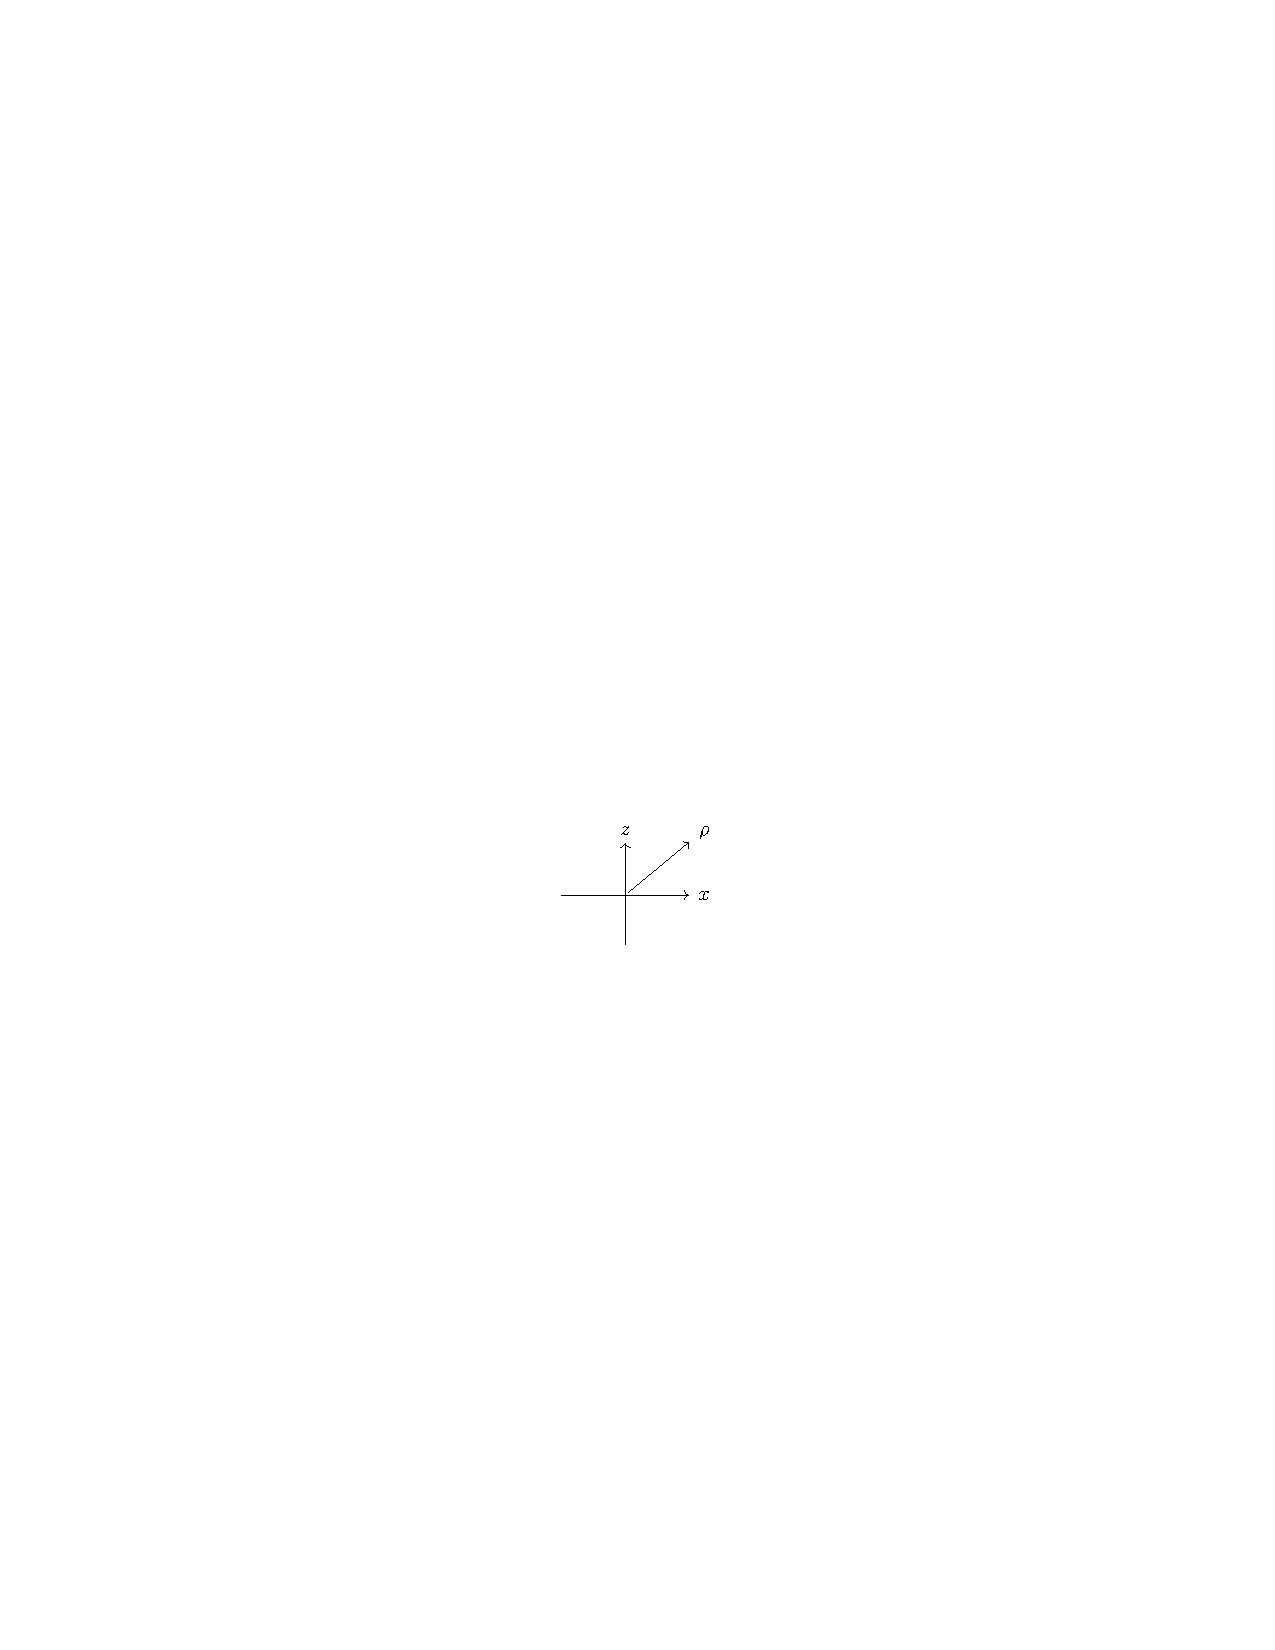
\includegraphics[width=0.1902\linewidth]{images/diagram-5-56.pdf}}}.}
从 $x$ 的方向向 $z$ 的方向穿过它。先取 $f_{\mathfrak p}=1+t^2x^{-1}z^{-1}$，则 $\Theta_{\mathfrak p}$ 映为
\Eq{5.57}{x\longmapsto(1+t^2x^{-1}z^{-1})x,\qquad z\longmapsto(1+t^2x^{-1}z^{-1})^{-1}z.}
\end{example}
\examnum{6}\begin{example}\label{ex:5.6}
传播中的壁沿余维二的多面体子集相交，这些子集称为\Term{jiehebu}{接合部}。采用下图的记号：
\Eq{5.58}{\vcenter{\hbox{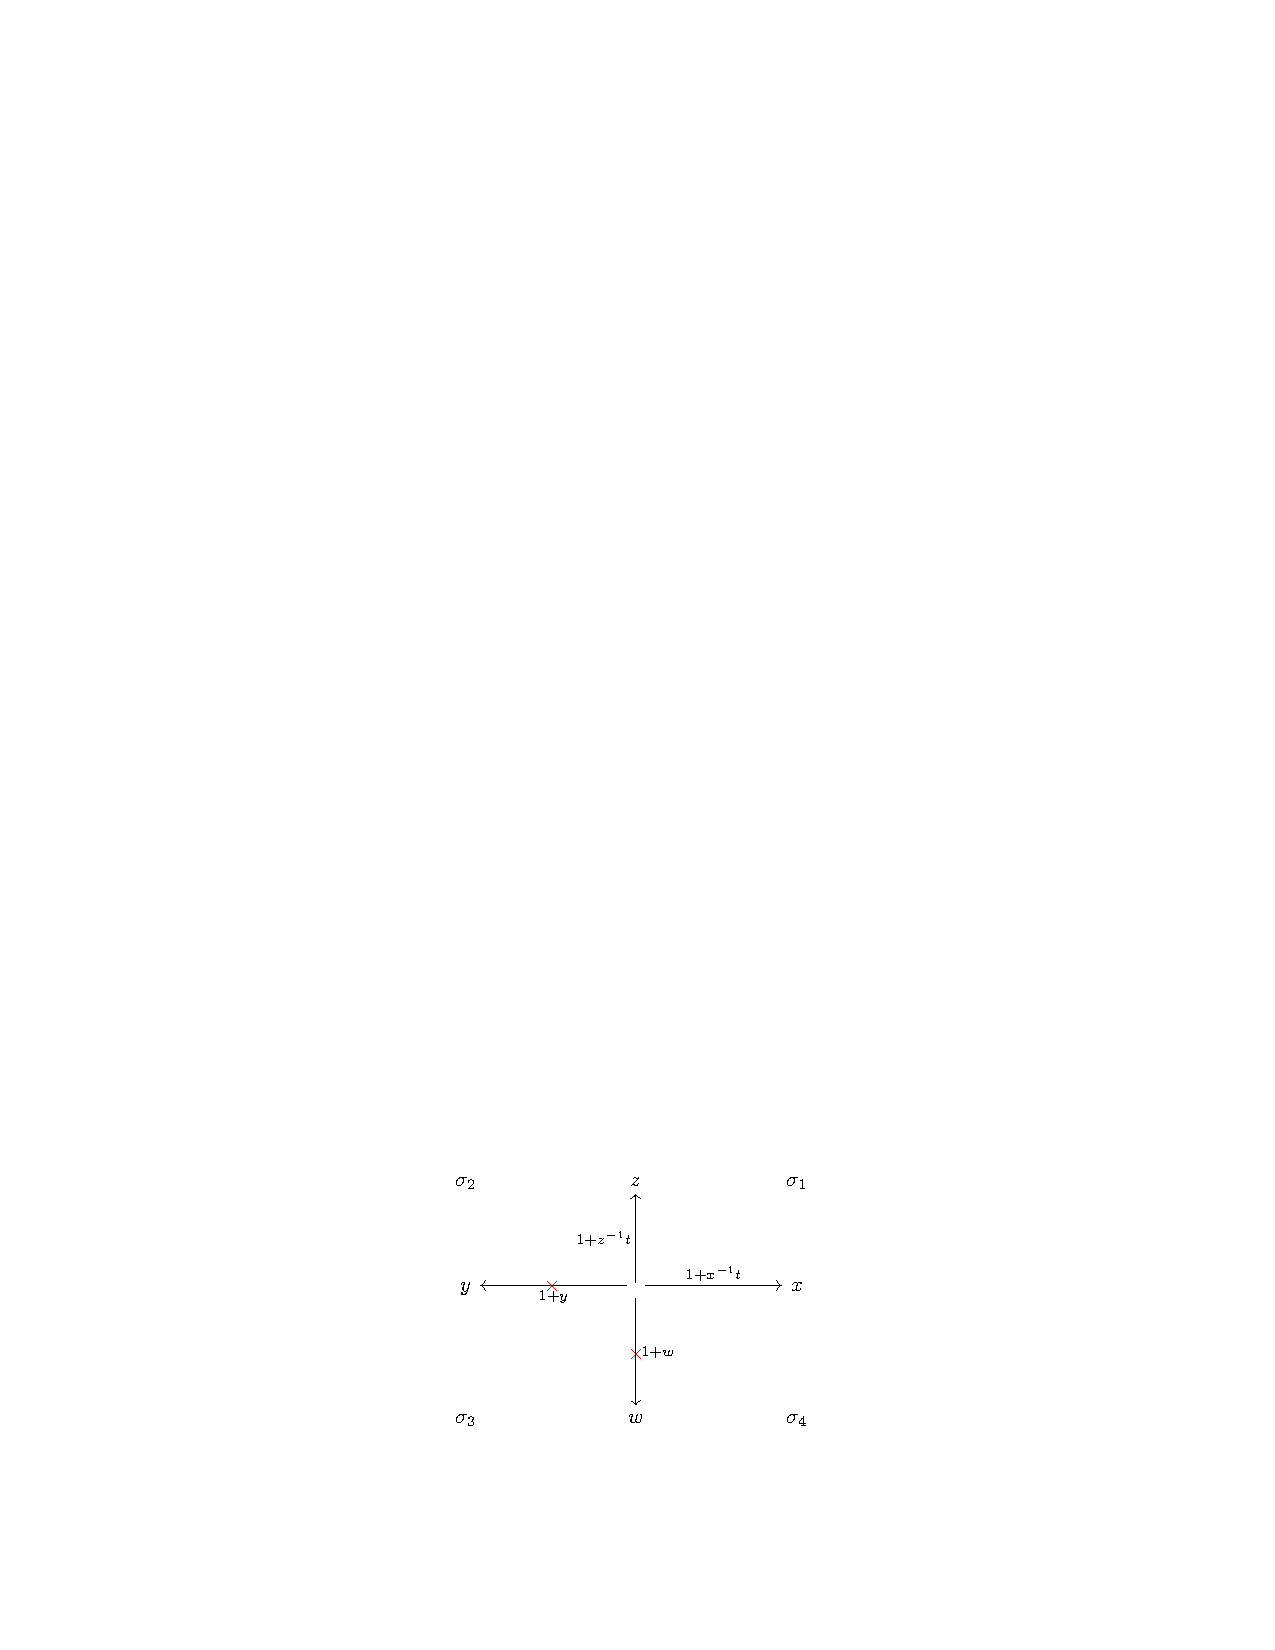
\includegraphics[width=0.4343\linewidth]{images/diagram-5-58.pdf}}}.}
\SourcePage{91}
依次穿过各壁，得到
\Eq{5.59}{\begin{aligned}x&\longmapsto(1+w)x\\&\longmapsto\bigl(1+(1+y)^{-1}w\bigr)x\\&\longmapsto\bigl(1+(1+(1+w)y)^{-1}w\bigr)(1+w)^{-1}x\\&\longmapsto\underbrace{\bigl(1+(1+(1+(1+y)w)y)^{-1}(1+y)w\bigr)(1+(1+y)w)^{-1}x}_{g}.\end{aligned}}
这个式子看上去很复杂，但实际上
\Eq{5.60}{g=\bigl(1+((1+y)+(1+y)wy)^{-1}(1+y)w\bigr)(1+(1+y)w)^{-1}x,}
\Eq{5.61}{g=\bigl(1+(1+wy)^{-1}w\bigr)(1+w+wy)^{-1}x,}
\Eq{5.62}{g=(1+wy)^{-1}(1+wy+w)(1+w+wy)^{-1}x,}
\Eq{5.63}{g=(1+wy)^{-1}x.}
因此，为使它相容，必须在右上方的对角线方向插入一面壁，其函数为
\Eq{5.64}{1+wy.}
这个理论的巧妙之处在于，无论从哪个单项式开始，该修正都有效。
\end{example}
Kontsevich–Soibelman 的观察如下。假定所有真壁的函数模 $t$ 均为 $1$，且绕接合部逆时针穿越一周的复合满足
\Eq{5.65}{\Theta=\underbrace{\Theta_{\mathfrak p_1}\cdots\Theta_{\mathfrak p_r}}_{\text{逆时针}}\equiv\id\pmod{t^{k+1}}.}
则可按出射方向插入函数为 $1+ct^{k+1}z^m$ 的壁，使
\Eq{5.66}{\prod\Theta_{\mathfrak p}\equiv\id\pmod{t^{k+2}}.}
这一插入在壁结构等价的意义下唯一。
\subsection{构造删去余维二轨迹后的\texorpdfstring{$\mathcal X^\circ$}{X°}}
回忆，目标是从 $(B,\mathscr P,\varphi)$ 与 $f_\rho$ 构造
\Eq{5.67}{\begin{gathered}\mathcal X^k\longrightarrow S_k=\Spec\CC[t]/(t^{k+1}),\\(\mathcal X^k)_0=X_0=\bigcup\text{环面簇}.\end{gathered}}
假定 $\mathscr S$ 在余维零和余维一处相容，定义
\Eq{5.68}{\mathcal X^\circ=\varinjlim\{\Spec R_e,\Spec R_{\mathfrak u}\},}
其中粘合使用壁穿越以及对 $e\subset\mathfrak u$ 的典范局部化 $R_e\to R_{\mathfrak u}$。
取 $B\setminus\bigcup_{\mathfrak p\in\mathscr S}\mathfrak p$ 的连通分支的闭包，不妨通过细分使它们凸，记为腔室 $\mathfrak u\subseteq\sigma$，并令 $R_{\mathfrak u}=R_\sigma$。相交于余维一处时，
\Eq{5.69}{R_e=A[\Lambda_e][z_+,z_-]/(z_+z_--f_e t^{\kappa_\rho}).}
\SourcePage{92}
\subsection{所有余维中的相容性与折线}
现在考虑\Term{zhexian}{折线} $\beta$。归纳地，在穿过壁 $\mathfrak p_j$ 时展开
\Eq{5.70}{\Theta_{\mathfrak p_j}(b_{j-1}z^{m_{j-1}})=\sum_i a_iz^{m_i},}
再从中选择下一段所携带的单项式 $b_jz^{m_j}\in\{a_iz^{m_i}\}$。
\thmnum{definition}{5}\begin{definition}\label{def:5.5}
若局部对折线求和能给出良定义的函数，则称壁结构 $\mathscr S=\{\mathfrak p\}$ 相容。
\end{definition}
\examnum{7}\begin{example}\label{ex:5.7}
设 $m_0=(-1,0)$，且 $z^{m_0}=x$。相应折线如下：
\Eq{5.71}{\vcenter{\hbox{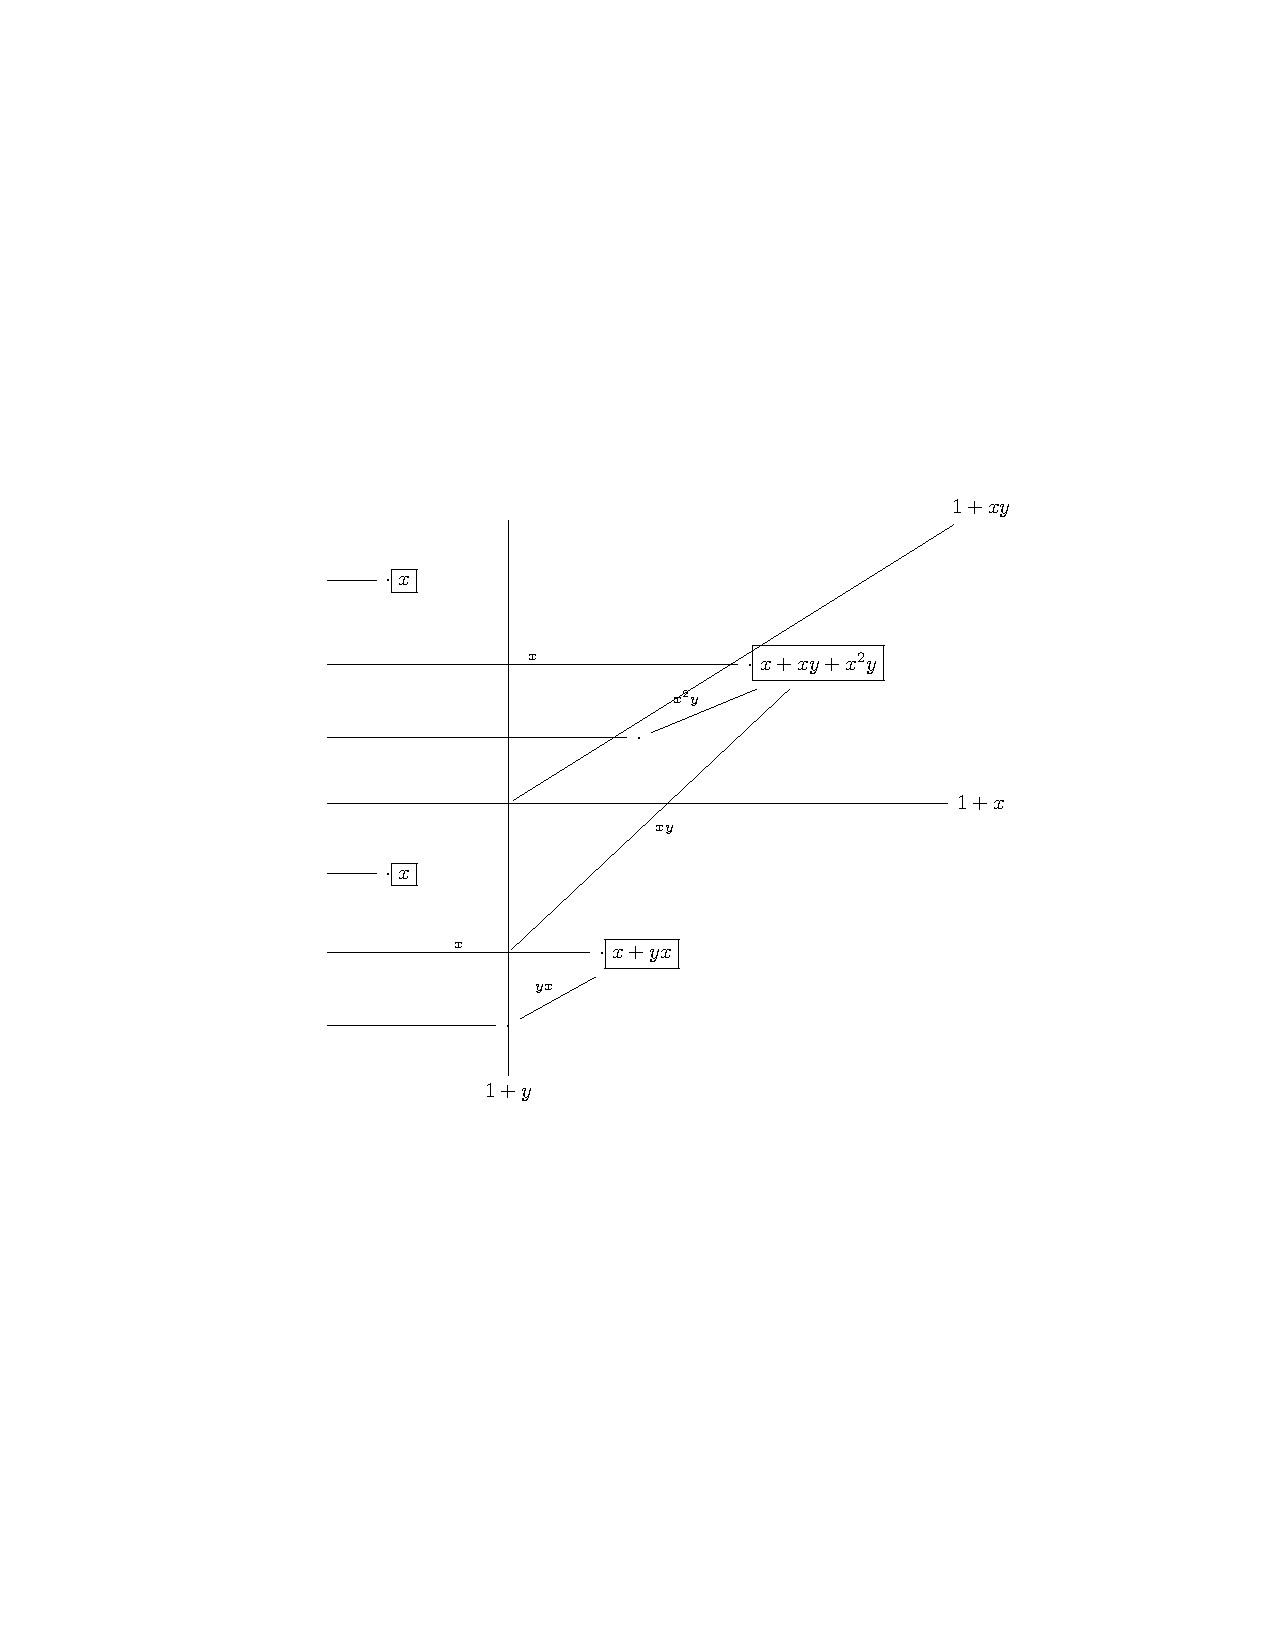
\includegraphics[width=0.8384\linewidth]{images/diagram-5-71.pdf}}}.}
\end{example}
\subsection{典范函数：广义\texorpdfstring{$\theta$}{θ}函数}
设 $\mathscr S$ 在余维不超过二处相容，$m$ 为一个渐近整向量场。用同样的构造，对折线求和得到
\Eq{5.72}{\vartheta_m\in\OO(\mathcal X^\circ).}
在 $\mathfrak u\subseteq\sigma$ 对应的 $R_{\mathfrak u}=A[\Lambda_\sigma]$ 上，定义
\Eq{5.73}{\vartheta_m=\sum_{\substack{\beta\text{ 的渐近单项式为 }z^m\\\text{终点为 }p}}b_\beta z^{m_\beta}.}
此表达式与同一腔室内的点 $p$ 的选择无关。
\subsection{构造\texorpdfstring{$\mathcal X\to\Spec A$}{X→Spec A}}
\SourcePage{93}
\thmnum{theorem}{7}\begin{theorem}\label{thm:5.7}
若 $\mathscr S$ 为 $(B,\mathscr P,\varphi)$ 上的相容壁结构，则存在部分完备化 $\mathcal X\supset\mathcal X^\circ$，满足
\Eq{5.74}{X_0=\bigcup_{\sigma\in\mathscr P}P(\sigma).}
\end{theorem}
\begin{proof}
在这里考虑的仿射情形，所有胞腔都是锥，因而没有正维有界胞腔，此时
\Eq{5.75}{\mathcal X=\Spec\left(\bigoplus_{m\in B(\ZZ)}A\vartheta_m\right).}
一般情形下，对 $\OO_{\mathcal X^\circ}(-1)$ 的总空间应用仿射构造。这里使用了如下事实：若 $X$ 为射影簇，$L\to X$ 为 $\OO_X(-1)$ 的总空间，则
\Eq{5.76}{\bigoplus_{d\ge0}\Gamma(X,\OO_X(d))\simeq\Gamma(L,\OO_L).}
在 $B$ 的层面上，这相当于在 $B$ 上方取截断锥。
\end{proof}
\subsection{构造相容壁结构}
第一种方法见文献~\cite{ref16}。在顶点附近，$B$ 有仿射坐标图，因为 $\Delta\cap|\mathscr P[0]|=\varnothing$。此时 $\mathcal X$ 是 $\mathcal Y\to\check S$ 的镜像，而 $Y_0$ 为环面簇的并。这是一个通过\Term{sanshe}{散射}进行的归纳构造，需要初始数据 $f_{\rho,v}=f_\rho$ 在余维二处满足“局部刚性”。

第二种方法见文献~\cite{ref14}，它把散射解释为环面曲面上的相对 Gromov–Witten 理论。此时 $\mathcal X$ 是对数 Calabi–Yau 曲面对 $(Y,D)$ 的镜像，$\mathcal Y\to\check S$ 且 $\dim Y_0=2$。这导向了文献~\cite{ref13} 的结果，因此可看作一种混合方法。

在即将开展的工作中，将利用 $(Y,D)$ 或 $(\mathcal Y,Y_0)$ 上的对数 Gromov–Witten 理论，其中 $\mathcal Y$ 是全纯曲线的热带化之并。
\section{内蕴镜像映射}
此处插入 Siebert 教授几周前在几何研讨班上的报告。关键是通过带穿孔的 Gromov–Witten 理论，构造与 $(Y,D)$ 或 $\mathcal Y$ 镜像的齐次坐标环。这是允许负接触阶的对数 Gromov–Witten 不变量，构造无需显式使用壁结构。由此，可以完全控制镜像构造：通过 $X$ 上的对数 Gromov–Witten 理论，从 $(X,D)$ 得到 $\mathcal Y\to S'$；或者通过退化族 $\mathcal X\to S$ 的同类理论得到 $\mathcal Y\to S'$。这实际上是亏格零的闭弦理论。

在仿射情形，先取一对 $(Y,D)$，其中 $D=\bigcup_iD_i\subset Y$ 为正规交叉除子。要求数值等价
\Eq{5.77}{K_Y+D\equiv\sum_i a_iD_i,\qquad a_i\ge0.}
这是此处对对数 Calabi–Yau 所作的全部要求。\footnote{这是一种相当宽泛的对数 Calabi–Yau 概念。}
\examnum{8}\begin{example}\label{ex:5.8}
考虑 $\PP^2$。回忆，$B(\ZZ)$ 由三个 $\NN^2$ 的副本粘合而成。对 $a,b>0$ 的 $(a,b)$，对应的接触行为为 $u\mapsto(u^a,u^b)$。环的基元素与接触阶一一对应。乘法规则为
\Eq{5.78}{\vartheta_{m_1}\vartheta_{m_2}=\sum_pN_{m_1,m_2,p}\vartheta_p,}
其中 $N_{m_1,m_2,p}$ 计数与 $D$ 的接触阶为 $m_1,m_2,-p$ 的亏格零曲线。困难之处在于证明结合律。
\end{example}
\SourcePage{94}
对固有的 Calabi–Yau 退化族，有
\Eq{5.79}{\begin{tikzcd}\mathcal Y\arrow[d]\&Y_0\arrow[l,hook]\arrow[d]\\S\&\{0\}\arrow[l,hook],\end{tikzcd}}
然后有
\Eq{5.80}{\mathcal X=\operatorname{Proj}\left(\bigoplus_m A\vartheta_m\right).}
\Lecture{26}{2019年12月3日}
面临的挑战如下：
\begin{itemize}
\item 提取 Hodge 结构变分以及亏格零的闭 Gromov–Witten 不变量；
\item 同调镜像对称（HMS）；
\item 其他镜像现象，其中还有大量开放问题：
\begin{itemize}
\item $g>0$ 的情形：非交换结构、幻影可积性；
\item 超 Kähler 情形：AAB 膜与几何 Langlands 理论；
\item Donaldson–Thomas 理论。
\end{itemize}
\end{itemize}
